\part{Calculos Manuales}

\section{Teoria}
\subsection{Líneas de flujo}
Las líneas de flujo representan los caminos que siguen las partículas de agua mientras se mueven a través de un medio poroso. Estas líneas son perpendiculares a las líneas equipotenciales y a las líneas de corriente. Las líneas de flujo son paralelas a la dirección del flujo de agua subterránea.
\subsection{Líneas Equipotenciales}
Las líneas equipotenciales representan zonas en donde el potencial hidráulico es constante. Esto significa, que no hay diferencia de energía entre dos puntos conectados por una línea equipotencial. Estas líneas sirven para poder visualizar la dirección del flujo de agua subterránea.
\subsection{Presión de Poros}

\subsection{Presión en Ataguía}
\subsubsection{Presión Total}
\subsubsection{Presión Efectiva}
\subsubsection{Estabilidad}
\section{Resultados}

\subsection{Diagramas Escala 1:200}

\begin{figure}[H]
    \centering
    \begin{minipage}{0.32\textwidth}
        \centering
        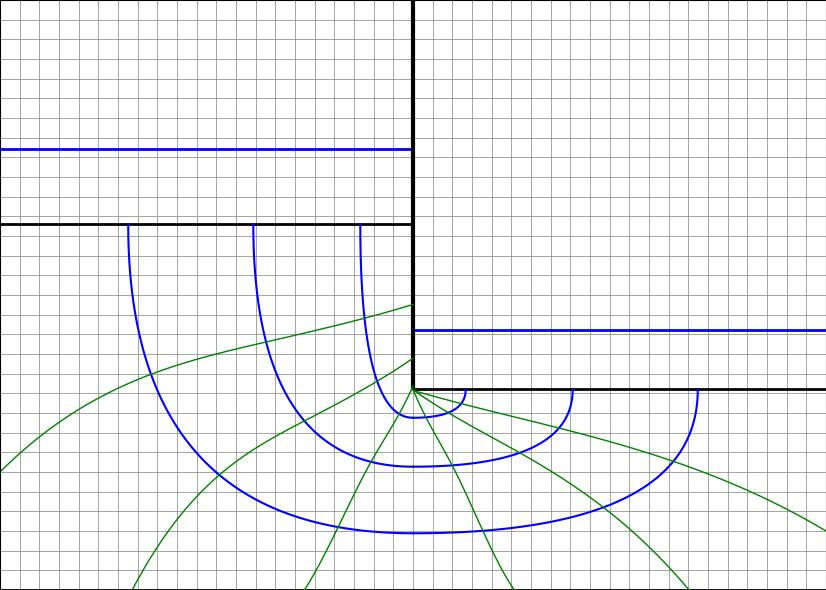
\includegraphics[width=\textwidth]{GRAFICOS/caso_1.jpg}
        \caption{Caso 1}
    \end{minipage}
    \begin{minipage}{0.32\textwidth}
        \centering
        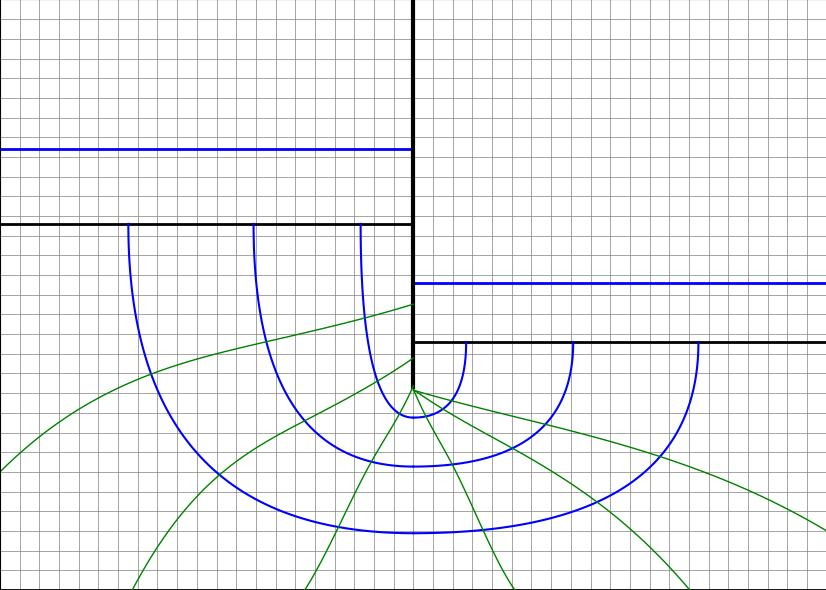
\includegraphics[width=\textwidth]{GRAFICOS/caso_2.jpg}
        \caption{Caso 2}
    \end{minipage}
    \begin{minipage}{0.32\textwidth}
        \centering
        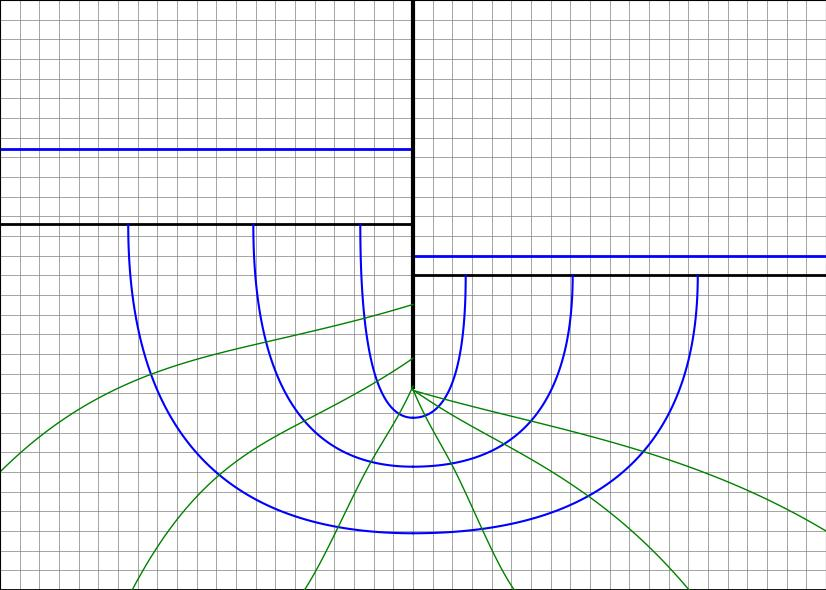
\includegraphics[width=\textwidth]{GRAFICOS/caso_3.jpg}
        \caption{Caso 3}
    \end{minipage}
  \end{figure}

\subsection{Presion de Poros}

\subsubsection{Distribucion Presiones}

\begin{figure}[H]
    \centering
    \begin{minipage}{0.32\textwidth}
        \centering
        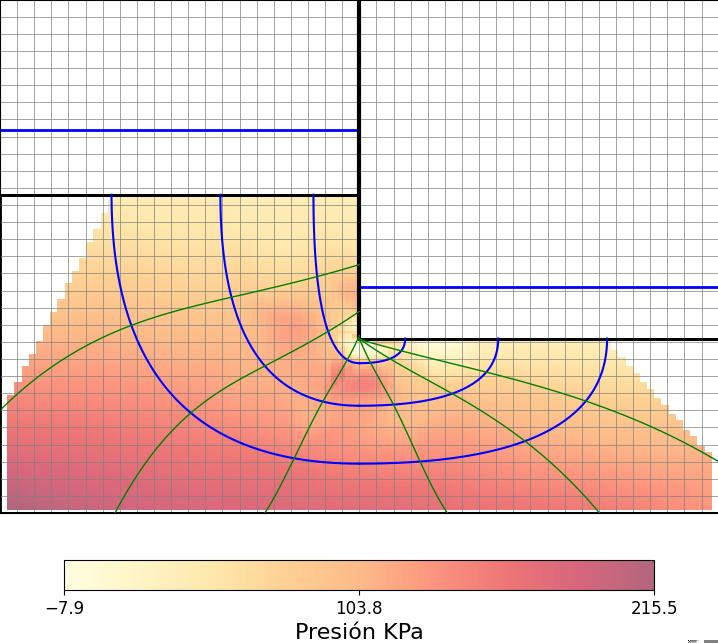
\includegraphics[width=\textwidth]{GRAFICOS/caso_1_presion_poros.jpg}
        \caption{Caso 1 Presion Poros}
    \end{minipage}
    \begin{minipage}{0.32\textwidth}
        \centering
        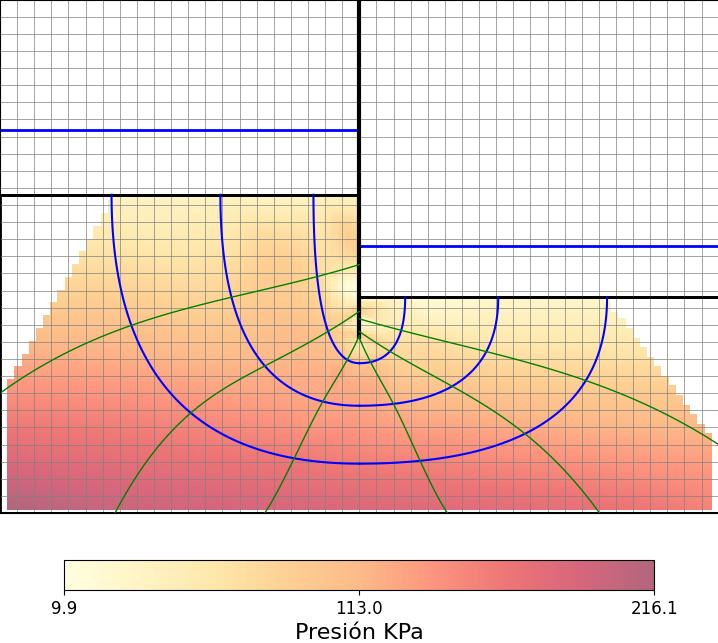
\includegraphics[width=\textwidth]{GRAFICOS/caso_2_presion_poros.jpg}
        \caption{Caso 2 Presion Poros}
    \end{minipage}
    \begin{minipage}{0.32\textwidth}
        \centering
        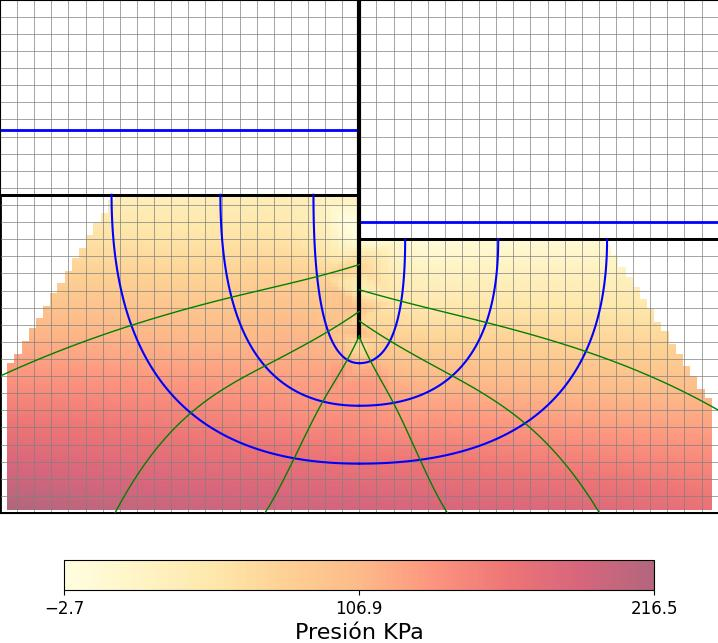
\includegraphics[width=\textwidth]{GRAFICOS/caso_3_presion_poros.jpg}
        \caption{Caso 3 Presion Poros}
    \end{minipage}
\end{figure}

\subsubsection{Presiones Totales}

\begin{figure}[H]
    \centering
    \begin{minipage}{0.32\textwidth}
        \centering
        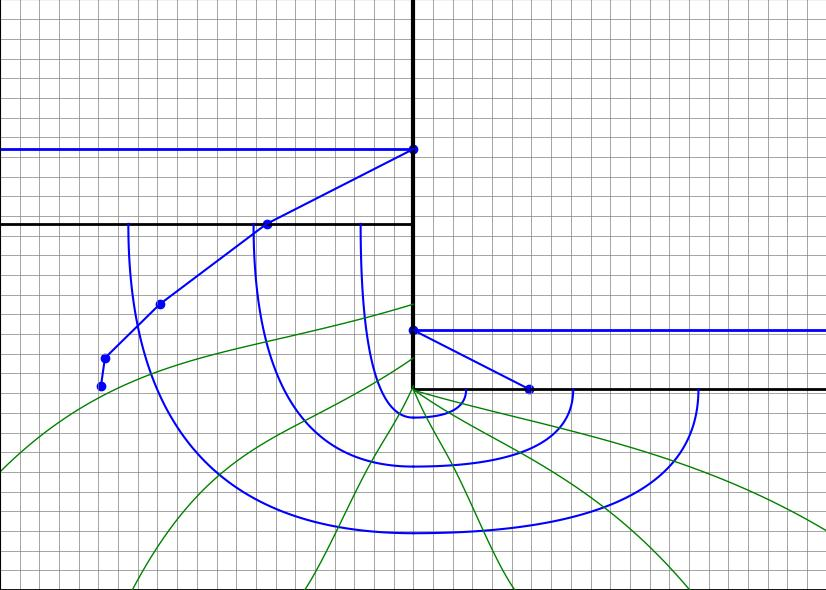
\includegraphics[width=\textwidth]{GRAFICOS/caso_1_presion_ataguia_total.jpg}
        \caption{Caso 1 Presion Ataguia Total}
    \end{minipage}
    \begin{minipage}{0.32\textwidth}
        \centering
        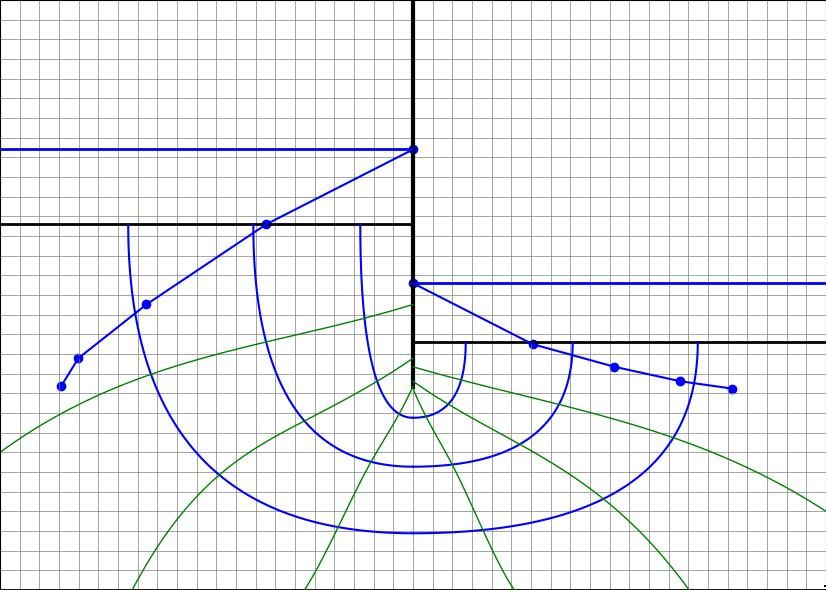
\includegraphics[width=\textwidth]{GRAFICOS/caso_2_presion_ataguia_total.jpg}
        \caption{Caso 2 Presion Ataguia Total}
    \end{minipage}
    \begin{minipage}{0.32\textwidth}
        \centering
        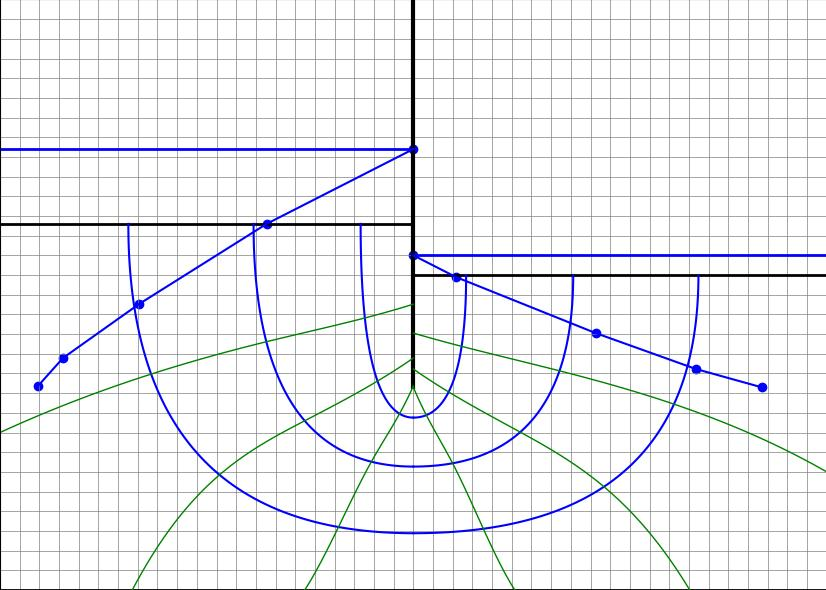
\includegraphics[width=\textwidth]{GRAFICOS/caso_3_presion_ataguia_total.jpg}
        \caption{Caso 3 Presion Ataguia Total}
    \end{minipage}
\end{figure}

\subsubsection{Presiones Efectivas}

\begin{figure}[H]
    \centering
    \begin{minipage}{0.32\textwidth}
        \centering
        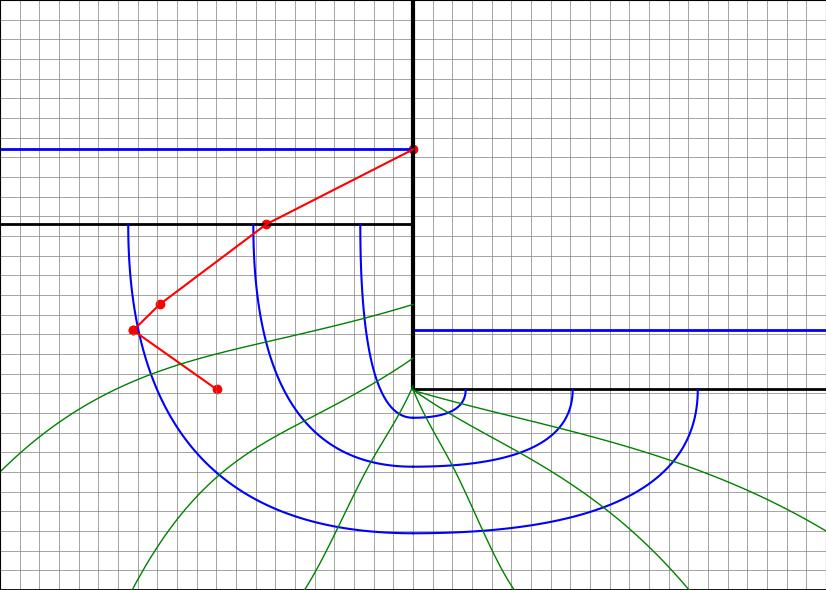
\includegraphics[width=\textwidth]{GRAFICOS/caso_1_presion_ataguia_neta.jpg}
        \caption{Caso 1 Presion Ataguia Neta}
    \end{minipage}
    \begin{minipage}{0.32\textwidth}
        \centering
        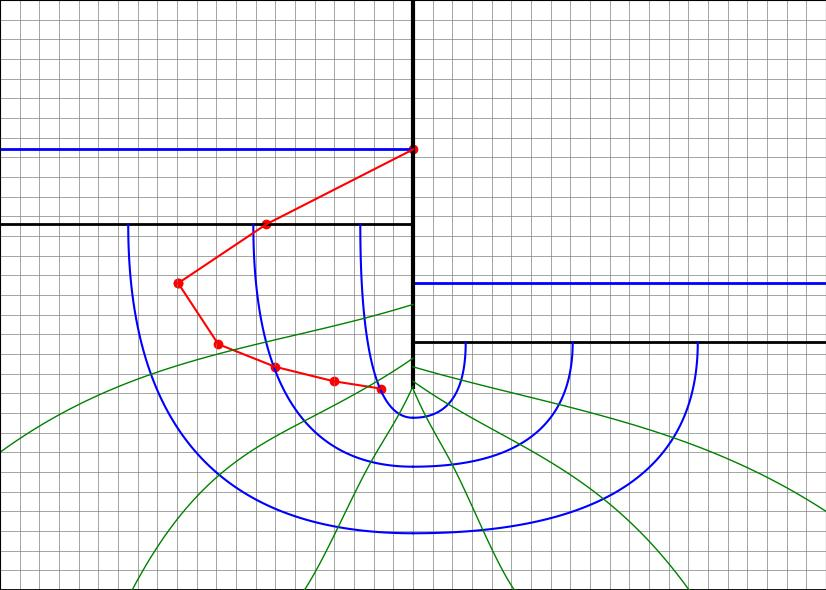
\includegraphics[width=\textwidth]{GRAFICOS/caso_2_presion_ataguia_neta.jpg}
        \caption{Caso 2 Presion Ataguia Neta}
    \end{minipage}
    \begin{minipage}{0.32\textwidth}
        \centering
        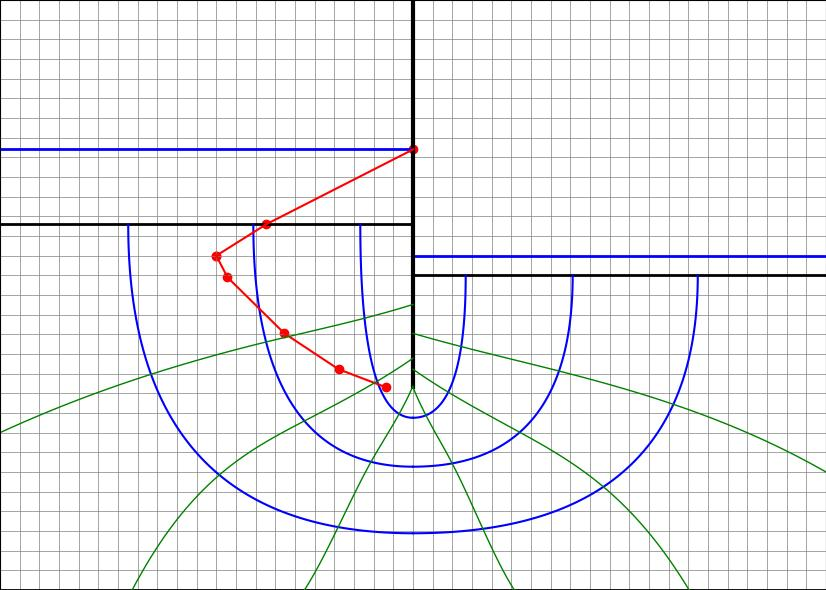
\includegraphics[width=\textwidth]{GRAFICOS/caso_3_presion_ataguia_neta.jpg}
        \caption{Caso 3 Presion Ataguia Neta}
    \end{minipage}
\end{figure}

\subsubsection{Estabilidad}

\begin{figure}[H]
    \centering
    \begin{minipage}{0.32\textwidth}
        \centering
        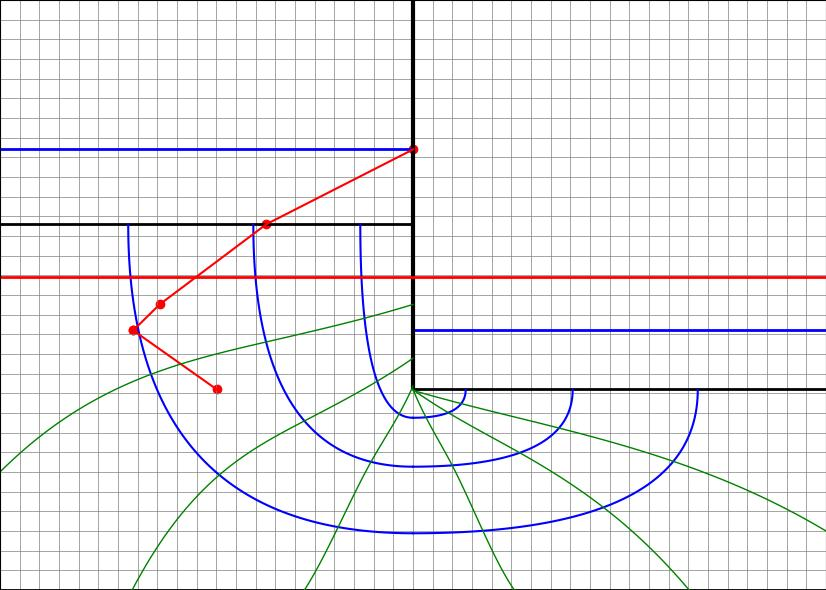
\includegraphics[width=\textwidth]{GRAFICOS/caso_1_centroide_y.jpg}
        \caption{Caso 1 Centroide}
    \end{minipage}
    \begin{minipage}{0.32\textwidth}
        \centering
        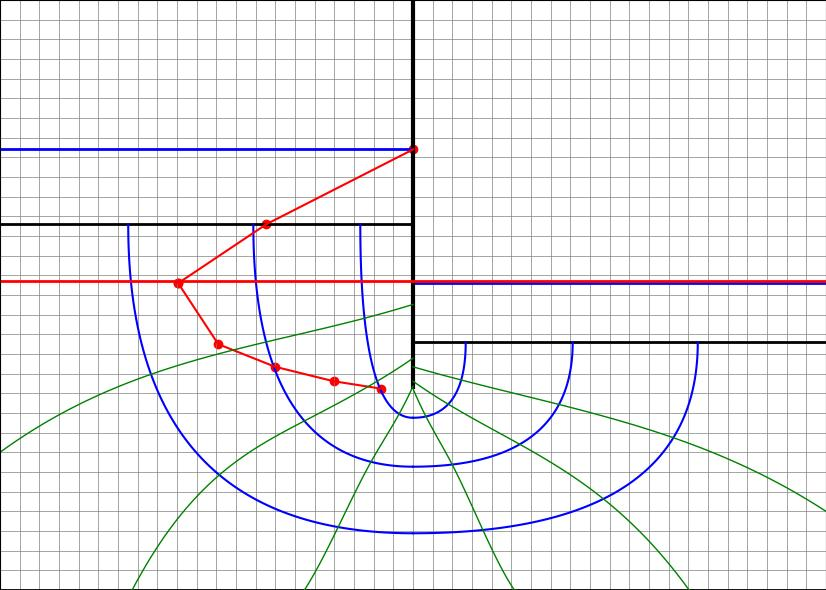
\includegraphics[width=\textwidth]{GRAFICOS/caso_2_centroide_y.jpg}
        \caption{Caso 2 Centroide}
    \end{minipage}
    \begin{minipage}{0.32\textwidth}
        \centering
        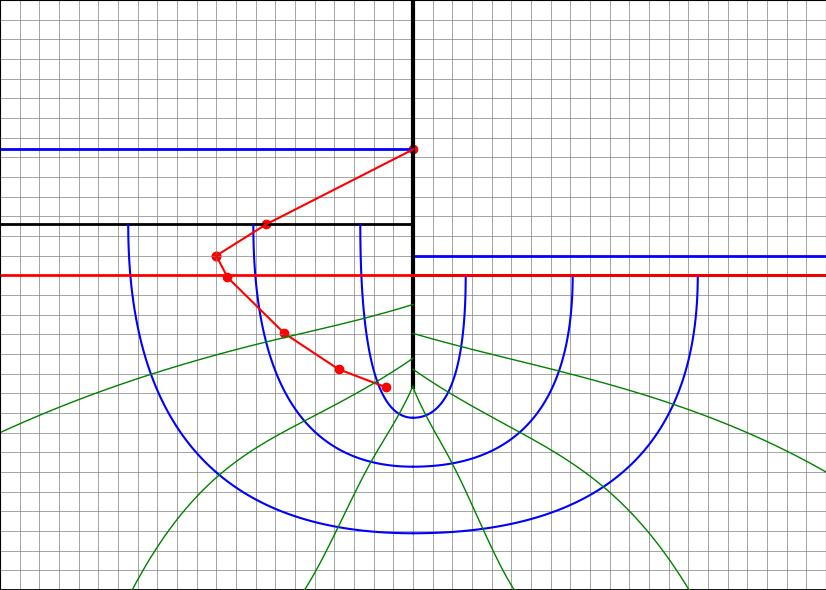
\includegraphics[width=\textwidth]{GRAFICOS/caso_3_centroide_y.jpg}
        \caption{Caso 3 Centroide}
    \end{minipage}
\end{figure}


